% Digital Logic Report Template
% Created: 2020-01-10, John Miller

%==========================================================
%=========== Document Setup  ==============================

% Formatting defined by class file
\documentclass[11pt]{article}

% ---- Document formatting ----
\usepackage[margin=1in]{geometry}	% Narrower margins
\usepackage{booktabs}				% Nice formatting of tables
\usepackage{graphicx}				% Ability to include graphics

%\setlength\parindent{0pt}	% Do not indent first line of paragraphs 
\usepackage[parfill]{parskip}		% Line space b/w paragraphs
%	parfill option prevents last line of pgrph from being fully justified

% Parskip package adds too much space around titles, fix with this
\RequirePackage{titlesec}
\titlespacing\section{0pt}{8pt plus 4pt minus 2pt}{3pt plus 2pt minus 2pt}
\titlespacing\subsection{0pt}{4pt plus 4pt minus 2pt}{-2pt plus 2pt minus 2pt}
\titlespacing\subsubsection{0pt}{2pt plus 4pt minus 2pt}{-6pt plus 2pt minus 2pt}

% ---- Hyperlinks ----
\usepackage[colorlinks=true,urlcolor=blue]{hyperref}	% For URL's. Automatically links internal references.

% ---- Code listings ----
\usepackage{listings} 					% Nice code layout and inclusion
\usepackage[usenames,dvipsnames]{xcolor}	% Colors (needs to be defined before using colors)

% Define custom colors for listings
\definecolor{listinggray}{gray}{0.98}		% Listings background color
\definecolor{rulegray}{gray}{0.7}			% Listings rule/frame color

% Style for Verilog
\lstdefinestyle{Verilog}{
	language=Verilog,					% Verilog
	backgroundcolor=\color{listinggray},	% light gray background
	rulecolor=\color{blue}, 			% blue frame lines
	frame=tb,							% lines above & below
	linewidth=\columnwidth, 			% set line width
	basicstyle=\small\ttfamily,	% basic font style that is used for the code	
	breaklines=true, 					% allow breaking across columns/pages
	tabsize=3,							% set tab size
	commentstyle=\color{gray},	% comments in italic 
	stringstyle=\upshape,				% strings are printed in normal font
	showspaces=false,					% don't underscore spaces
}

% How to use: \Verilog[listing_options]{file}
\newcommand{\Verilog}[2][]{%
	\lstinputlisting[style=Verilog,#1]{#2}
}




%======================================================
%=========== Body  ====================================
\begin{document}

\title{ELC 2137 Lab 05: Intro to Verilog}
\author{Yiting Wang}

\maketitle


\section*{Summary}

In this Lab we are going to describe digital circuits with code,  or a  hardware description language  (HDL). That's because before we built digital circuits using hardware devices.  This becomes cumbersome very quickly.  It would be possible to draw circuit schematics in soft-ware then “program” them onto a device.  This is easier/faster than physically wiring by hand and allows for much larger, more complicated designs, but still requires a significant amount of click-and-place. \\



\section*{Q\&A}

\begin{enumerate}
	\item Comment on whether the simulations match the expected output values? \\
	In the half adder and the full adder, the simulations match the expected output values; but in the two bit adder/subtractor, the simulation doesn't match the expected output values. \\
	\item What is one thing that you still don’t understand about Verilog? \\
	I don't know a lot of it casue I am a beginner, but I think I understand all the knowledge in this lab. \\
\end{enumerate}



\section*{Results}

Firgure 1 is the block diagrams for half adder module. \\
\begin{figure}[ht]\centering    
	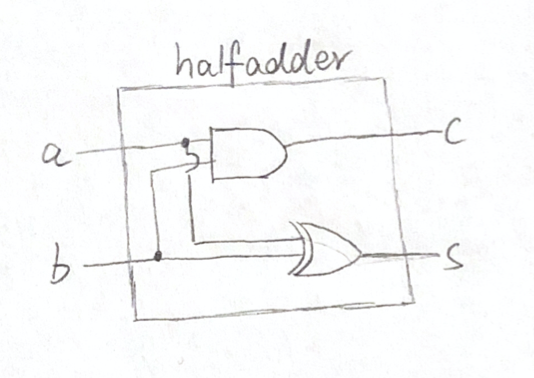
\includegraphics[width=0.5\textwidth]{halfadder}    
	\caption{This is the block diagrams for half adder module.}    
	\label{fig:halfadder}
\end{figure}

Firgure 2 is the simulation waveform and ERT of half adder, this simulation matches the expected output values, and the code about that is in the Code section. \\
\begin{figure}[ht]\centering
	\begin{tabular}{l|rrrr}
		Time (ns): & 0 & 10 & 20 & 30 \\
		\midrule
		a & 0 & 0 & 1 & 1 \\
		b & 0 & 1 & 0 & 1 \\
		\midrule
		c & 0 & 0 & 0 & 1 \\
		s & 0 & 1 & 1 & 0 \\
		\bottomrule
	\end{tabular}\medskip
		
	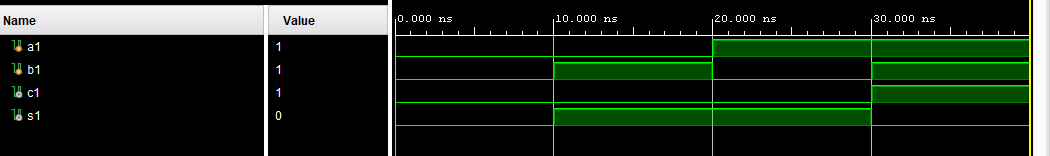
\includegraphics[width=1\textwidth]{HalfAdderSimulation}
	\caption{the simulation waveform and ERT of half adder}
	\label{fig:HalfAdderSimulation}
\end{figure}

Firgure 3 is the block diagrams for full adder module. \\
\begin{figure}[ht]\centering    
	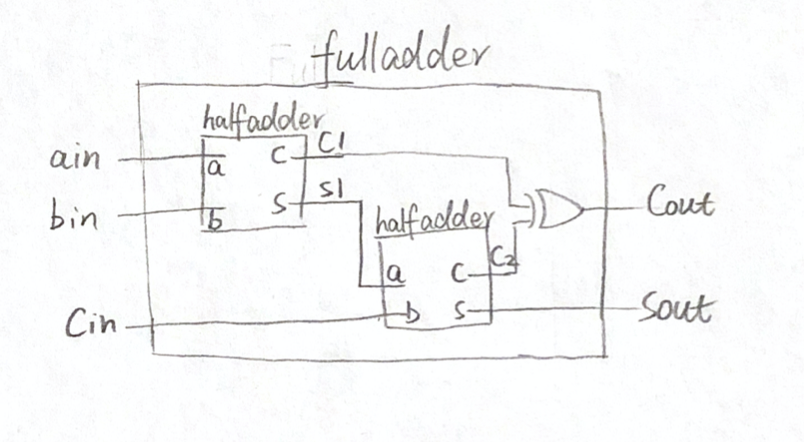
\includegraphics[width=0.5\textwidth]{fulladder}    
	\caption{This is the block diagrams for full adder module.}    
	\label{fig:fulladder}
\end{figure}

Firgure 4 is the simulation waveform and ERT of full adder, this simulation matches the expected output values, and the code about that is in the Code section. \\
\begin{figure}[ht]\centering
	\begin{tabular}{l|rrrr|rrrr}
		Time (ns): & 0 & 10 & 20 & 30 & 40 & 50 & 60 & 70\\
		\midrule
		cin & 0 & 0 & 0 & 0 & 1 & 1 & 1 & 1 \\
		a & 0 & 0 & 1 & 1 & 0 & 0 & 1 & 1 \\
		b & 0 & 1 & 0 & 1 & 0 & 1 & 0 & 1 \\
		\midrule
		c & 0 & 0 & 0 & 1 & 0 & 1 & 1 & 1 \\
		s & 0 & 1 & 1 & 0 & 1 & 0 & 0 & 1\\
		\bottomrule
	\end{tabular}\medskip
		
	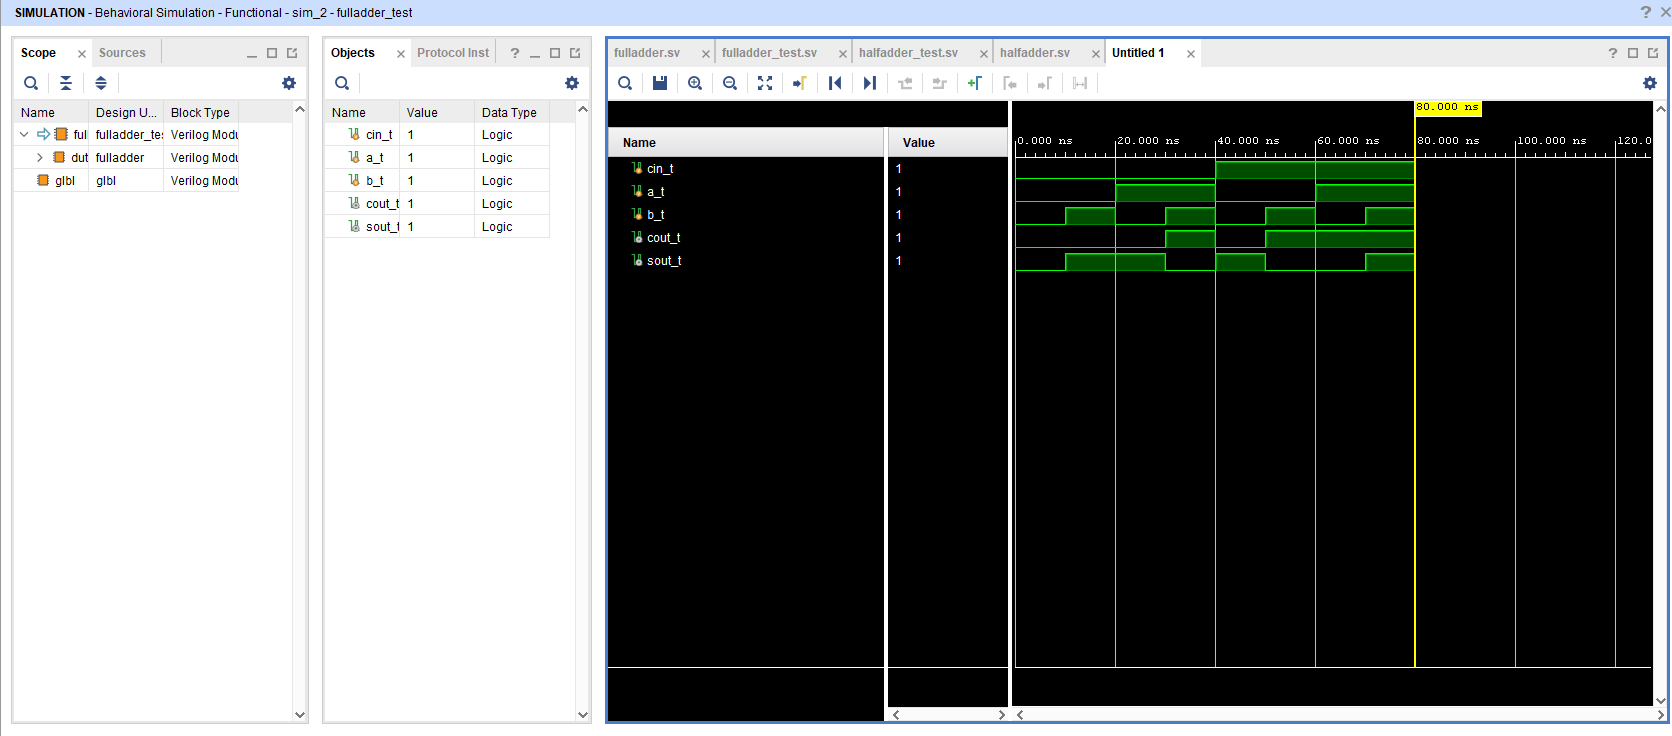
\includegraphics[width=1\textwidth]{FullAdderSimulation}
	\caption{the simulation waveform and ERT of full adder}
	\label{fig:FullAdderSimulation}
\end{figure}

Firgure 5 is the block diagrams for two bit adder/subtractor module. \\
\begin{figure}[ht]\centering    
	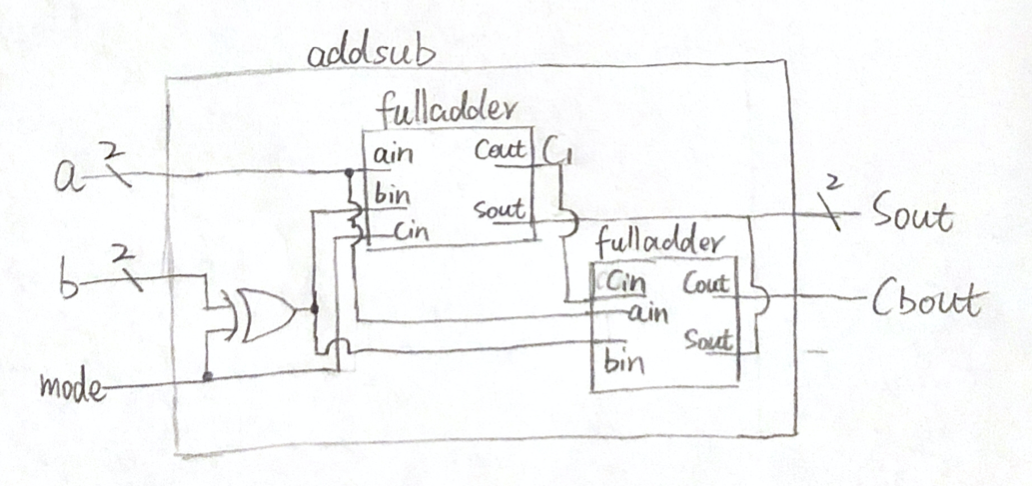
\includegraphics[width=0.5\textwidth]{addsub}    
	\caption{This is the block diagrams for two bit adder/subtractor module.}    
	\label{fig:addsub}
\end{figure}

Firgure 6 is the simulation waveform and ERT of two bit adder/subtractor, this simulation doesn't match the expected output values, and the code about that is in the Code section. \\
\begin{figure}[ht]\centering
	\begin{tabular}{l|rrrr|rrrr|rrrr|rr}
		Time (ns): & 0 & 10 & 20 & 30 & 40 & 50 & 60 & 70 & 80 & 90 & 100 & 110 & 120 & 130 \\
		\midrule
		A1A0 & 00 & 00 & 00 & 00 & 01 & 10 & 10 & 00 & 00 & 00 & 00 & 01 & 10 & 10 \\
		B1B0 & 00 & 01 & 10 & 11 & 01 & 01 & 00 & 00 & 01 & 10 & 11 & 01 & 01 & 00 \\
		mode & 0 & 0 & 0 & 0 & 0 & 0 & 0 & 1 & 1 & 1 & 1 & 1 & 1 & 1 \\
		\midrule
		c & 0 & 0 & 0 & 0 & 0 & 0 & 0 & 0 & 1 & 1 & 1 & 0 & 0 & 0 \\
		s1 & 0 & 0 & 1 & 1 & 1 & 1 & 1 & 0 & 1 & 1 & 0 & 0 & 0 & 1 \\
		s0 & 0 & 1 & 0 & 1 & 0 & 1 & 0 & 0 & 1 & 0 & 1 & 0 & 1 & 0 \\
		\bottomrule
	\end{tabular}\medskip
		
	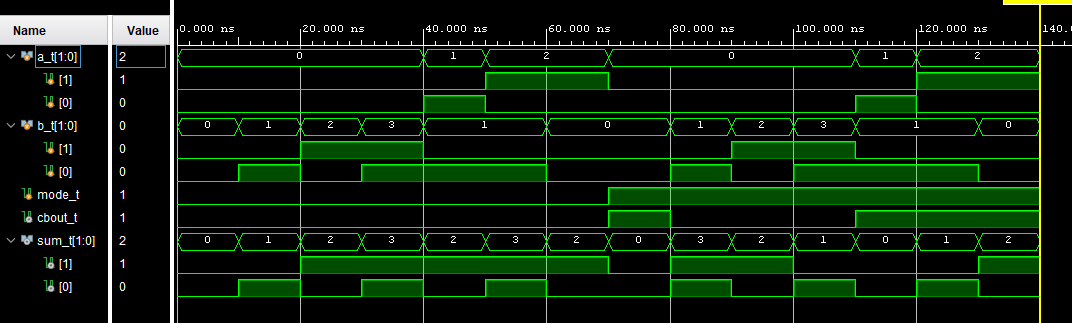
\includegraphics[width=1\textwidth]{AddSubSimulation}
	\caption{the simulation waveform and ERT of two bit adder/subtractor}
	\label{fig:AddSubSimulation}
\end{figure}



\section*{Code}

\subsection*{File Inclusion}
\Verilog[caption=Half Adder Verilog code,label=code:file_ex]{halfadder.sv}

\subsection*{File Inclusion}
\Verilog[caption=Half Adder Test Benches Verilog code,label=code:file_ex]{halfadder_test.sv}

\subsection*{File Inclusion}
\Verilog[caption=Full Adder Verilog code,label=code:file_ex]{fulladder.sv}

\subsection*{File Inclusion}
\Verilog[caption=Full Adder Test Benches Verilog code,label=code:file_ex]{fulladder_test.sv}

\subsection*{File Inclusion}
\Verilog[caption=Two Bit Adder/Aubtractor Verilog code,label=code:file_ex]{addsub.sv}

\subsection*{File Inclusion}
\Verilog[caption=Two Bit Adder/Aubtractor Test Benches Verilog code,label=code:file_ex]{addsub_test.sv}



\end{document}
